\documentclass{article}
\usepackage{mathtools}
\usepackage{indentfirst}
\usepackage{url}
\usepackage{listings}
\usepackage{color}
\usepackage[numbers]{natbib}
\usepackage{float}
\usepackage{hyperref}

\definecolor{mygreen}{rgb}{0,0.6,0}
\definecolor{mygray}{rgb}{0.5,0.5,0.5}
\definecolor{mymauve}{rgb}{0.58,0,0.82}

\begin{document}

\begin{titlepage}
  \centering
  
\includegraphics[width=0.5\textwidth]{nus}

  \LARGE Final Year Project

  \vspace{1cm}
  \Large Asian Option Pricing through Finite Difference Schemes

  \vspace{1cm}

  \Large Emmanuel Goh
  \vfill
  \large \today
\end{titlepage}

\tableofcontents

\newpage

\section{Introduction}

The Asian Option is an option whose payoff is dependent on the average price of the underlying asset over a period of time. These come in fixed strike and floating strike variants. Many different methods of pricing exist, among which include closed-form approximations, lattice methods, as well as Monte Carlo simulations. Each have distinct advantages over the other.

In this paper, we price an Asian calls of both the fixed and floating strike variety using the Implicit Finite Difference Scheme method, applying transformations used by 5 different Partial Differential Equations to construct the Finite Difference Grid. Namely, these transformations will be referred to as the Rogers-Shi, Vecer, Dubois-Leli\`evre, New and New-Vecer equations.

\section{Definitions}
The following variables will be used throughout the paper. Where necessary, mathematical definitions will follow later.
\begin{table}[H]
  \begin{tabular}{|c|c|}
    \hline
    \textbf{Description} & \textbf{Variable Name} \\ \hline
    Stock Price & \(S\) \\
    Strike Price & \(K\)\\
    Average Price & \(A\) \\
    Time ago which averaging started & \(t_0\) \\
    Remaining lifespan of the Option & \(T\) \\
    Risk Free Rate & \(r\) \\
    Dividend Rate & \(\delta\) \\
    \hline
  \end{tabular}
  \caption{Variables used in various equations}
  \label{table:name}
\end{table}

\section{Finite Difference Schemes}

The Finite Difference Scheme method allows for flexibility between accuracy and time. Monte Carlo methods are heavily dependent on the number of paths to increase accuracy \cite{montecarlo}. For closed form approximations, no tradeoff can be made.

The Implicit Finite Difference Scheme is a modification of the Binomial Tree Method, whereby discretizing a grid over a continuous domain and setting particular boundary and terminal values allows us to iteratively recover the fair price of an option today.

\subsection{Binomial Tree Methods}
\begin{figure}[H]
  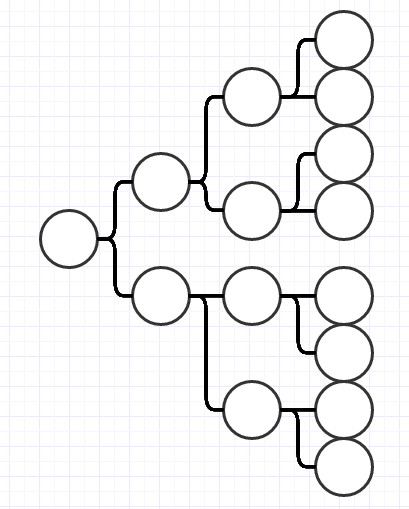
\includegraphics[width=0.5\textwidth]{btm}
  \caption{Binomial Tree Method}
  \label{figure:name}
\end{figure}

The Binomial Tree Method is based on the concept that the price of a stock can either move up or down with the probabilities \(p\) and \(1-p\) respectively. Then, by calculating the probability that any particular path is taken over a finite, discretized number of time points \(n\), we have \(2^n\) different terminal values, each with the probability of occuring \(p^k(1-p)^{n-k}\) where \(k\) is the number of upward movements. Discounting the expected payoff of the option then yields the fair price today. The major flaw in this design is that the time complexity of this naive method is \(O(2^n)\), which is unacceptable for any reasonable usage.

This then leads to a slightly improved method where the product of the upward and downward movements is 1. This causes the tree to simplify significantly, becoming the following figure.

\begin{figure}[H]
  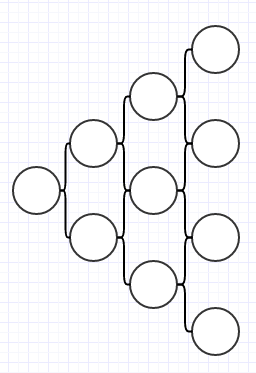
\includegraphics[width=0.5\textwidth]{btm_improved}
  \caption{Improved Binomial Tree Method}
  \label{figure:name}
\end{figure}

This reduces the complexity from the abovementioned to a respectable \(O(n)\) (noting we only need to get the values of the nodes on the rightmost). However, this method is heavily restricted by the assumptions we place on it, and is unable to retrieve accurate results.

\subsection{Finite Difference Schemes}
The Improved Binomial Tree Method however lays the foundation of for the explicit finite difference scheme. We see that the \(t_{n+1}\) price of a stock or option is influenced by the \(t_n\) price. Also, the payoff function of a option is clearly known. We then make reasonable assumptions about the highest possible and lowest possible price of a stock, and define appropriate boundary values. Then, discretizing a grid of \(n\) time points and \(m\) price (or state) points, we can iteratively recover the fair price of an option today, using relations between points on the grid that are governed by a discretized partial differential equation.

In this project, an implicit scheme is used, that is, the value of a point at \(t_n\) is influenced by points at both \(t_n\) and \(t_{n+1}\), thus a linear system of size \(m^2\) is solved at each iteration. This results in an overall compleixity of \(O(nm^3)\), which may be unimpressive, but significantly outperforms the Monte Carlo methods when requiring higher levels of accuracy. Here, the Crank-Nicholson discretization is applied to the 5 abovementioned equations, all of which are based on the assumptions of the Black-Scholes model.

\section{Derivation}

The payoff of the options for the fixed and floating strike calls are respectively \(max\{A_T - K, 0\}\) and \(max\{S_T - A_T, 0\}\), given the average price of a stock, which can be calculated by
\begin{equation}
  A_T = \frac{t_0A + \int_0^T S_t \mathrm{d}t}{t_0 + T}.
\end{equation}

Supposing that the stock price \(S\) follows Geometric Brownian Motion, we have

\begin{equation}
  \mathrm{d}S_t = \mu S_t \mathrm{d}t + \sigma S_t \mathrm{d}W_t.
\end{equation}

In the risk-neutral world, this comes to
\begin{equation}
  \mathrm{d}\tilde{S}_t = \mu \tilde{S}_t \mathrm{d}t + \sigma \tilde{S}_t \mathrm{d}W_t,
\end{equation}
where \(\tilde{S}_t = e^{-\delta(T-t)}S_t\).

For convenience purposes, we also define the function \(q(t)\) such that
\begin{equation}
  q(t) =
  \begin{dcases*}
    1 - e^{-(r-\delta)(T-t)} & \(r \neq \delta\) \\
    \frac{T-t}{t_0 + T} & \(r\) = \(\delta\)
  \end{dcases*},
\end{equation}

We obtain the value process of a self-financing portfolio with payoff \(A_T\), also known as the average asset in our situation here, using the following identity:

\begin{equation}
  E_P(\int_0^TS_u\textrm{d}u | \mathcal{F}_t) = \int_0^t S_u \textrm{d}u + \int_t^T S_te^{(r-\delta)(u-t)}\textrm{d}u,
\end{equation}

\begin{equation}
  A_t = e^{-r(T-t)}E_P(A_T|\mathcal{F}_T) = q(t)\tilde{S_t} + e^{-r(T-t)} \frac{t_0 A + \int_0^tS_u\mathrm{d}u}{t_0+T}.
\end{equation}

Using Ito's Lemma on the risk-neutral asset yields

\begin{equation}
 \textrm{d}(\frac{e^{rt}}{\tilde{S}_t}) = -\sigma \frac{e^{rt}}{\tilde{S}_t}\textrm{d}W_t^S,
\end{equation}
where \(W_t^S = W_t - \sigma t\).

We also define
\begin{equation}
  \xi_t =
  \begin{dcases*}
    a(t) + b(t) \frac{A_t - Ke^{-\delta(T-t)}}{\tilde{S_t}} & Fixed calls (in general) \\
    a(t) + b(t) \frac{A_t}{S_t} & Floating calls (in general) \\
    e^{-r(T-t)}\frac{S_t}{A_t} & New-Vecer fixed call \\
    \frac{S_t}{A_t} & New-Vecer floating call
  \end{dcases*}
\end{equation}
and make use of the following generic governing partial differential equation

\begin{equation}
  \phi_t + [\dot{a}(t) + \dot{b}(t)(\xi - a(t))/b(t)]\phi_\xi + \frac{1}{2}\sigma^2[a(t)+b(t)q(t) - \xi]^2\phi_{\xi\xi} = 0,
\end{equation}
where \(\phi(T, \xi) = f(\xi)\), and \(f(\xi)\) is defined as per the below table, and \(a(t)\) and \(b(t)\) are arbitrary functions.

\begin{table}[H]
  \begin{tabular}{|c|c|c|}
    \hline
    & Fixed Strike & Floating Strike \\
    \hline
    Calls & \(max\{(\xi - a(T))/b(T), 0\}\) & \(max\{(a(T) - \xi)/b(T) + 1, 0\}\) \\
    Puts & \(max\{(a(T) - \xi)/b(T ), 0\}\) & \(max\{(\xi - a(T))/b(T) - 1, 0\}\)\\
    \hline
  \end{tabular}
  \caption{Different possible values of \(f(\xi)\)}
\end{table}

\section{Partial Differential Equations}
We show the transformations used in the 5 different partial differential equations.

For the Rogers-Shi equation, taking \(a(t)\) = \(-b(t)q(t)\) and \(b(t) = -e^{(r-\delta)(T-t)}\), we have the partial differential equation

\begin{equation}
  \phi_t - ( (r-\delta)\xi + \frac{1}{t_0 + T} )\phi_\xi + \frac{1}{2}\sigma^2\xi^2\phi_{\xi\xi} = 0.
\end{equation}We note that in this case, the coefficients do not depend on time. This gives rise to an interesting optimization in the code later that results in a faster numerical runtime for pricing with this partial differential equation.

For the Vecer equation, taking \(a(t) = 0\) and \(b(t)=1\) yields

\begin{equation}
  \phi_t + \frac{1}{2}\sigma^2(q(t) - \xi)^2\phi_{\xi\xi} = 0.
\end{equation}

For the Dubois-Leli\`{e}vre equation, taking \(a(t) = \frac{t}{t_0 + T} - q(t)b(t)\) and \(b(t)=-e^{(r-\delta)(T-t)}\) yields

\begin{equation}
  \phi_t + (r-\delta)(\frac{t}{t_0 + T} - \xi)\phi_\xi + \frac{1}{2}\sigma^2(\frac{t}{t_0 + T} - \xi)^2\phi_{\xi\xi} = 0.
\end{equation}

For the New equation, taking \(a(t) = -q(t)b(t)\) and \(b(t) = 1\) yields

\begin{equation}
  \phi_t + \frac{e^{-(r-\delta)(T-t)}}{t_0 + T}\phi_\xi + \frac{1}{2}\sigma^2\xi^2\phi_{\xi\xi} = 0.
\end{equation}

Finally, for the New Vecer equation, for the floating strike case (Vecer 2014), using \(A_t\) as numeraire, we have \(\xi_t = \frac{\tilde{S}_t}{A_t}\). This eventually yields the partial differential equation % citation needed

\begin{equation}
  \phi_t + \frac{1}{2}\sigma^2\xi^2(q(t)\xi - 1)^2 \phi_{\xi\xi} = 0.
\end{equation}

\subsection{Boundary Conditions}
\begin{table}[H]
  \begin{tabular}{|c|c|c|}
    \hline
    & \(\xi \rightarrow \infty\) & \(\xi \rightarrow -\infty\) \\
    \hline
    \(b(t) > 0\) &  & \(\phi(t, \xi) \rightarrow 0\) \\
    \(b(t) < 0\) & \(\phi(t, \xi) \rightarrow 0\) & \\
    \hline
  \end{tabular}\\
  \begin{tabular}{|c|c|c|}
    \hline
    & \(\xi \ge a(t) + q(t)b(t)\) & \(\xi \le a(t) + q(t)b(t)\) \\
    \hline
    \(b(t) > 0\) & \(\phi(t, \xi) = \frac{\xi-a(t)}{b(t)} \) & \\
    \(b(t) < 0\) &  & \( \phi(t, \xi) = \frac{\xi-a(t)}{b(t)} \) \\
    \hline
  \end{tabular}
  \caption{Different Boundary Conditions}
\end{table}

\subsection{Rogers Shi Fixed Strike Calls}
We take
\begin{equation}
  \xi_t = q(t)e^{(r-\delta)(T-t)} - e^{(r-\delta)(T-t)}\frac{A_t - Ke^{-\delta(T-t)}}{\tilde{S_t}}.
\end{equation}

Then, we have \( a(t) = -q(t)b(t) \) and \(b(t) = -e^{-(r-\delta)(T-t)}\). The partial differential equation then becomes

\begin{equation}
  \phi_t - ( (r-\delta)\xi + \frac{1}{t_0 + T} ) \phi_\xi + \frac{1}{2}\sigma^2\xi^2\phi_{\xi\xi} = 0.
\end{equation}

Rogers and Shi show that the value of the option at time \(t\) is given by \(S_t\phi(t, \xi_t)\). We then solve the PDE with the following conditions:

\begin{equation}
  \phi(T, \xi) = 0, 0 \le \xi \le \xi_{max}
\end{equation}
\begin{equation}
  \phi(t, 0) = q(t) \\
\end{equation}
\begin{equation}
  \phi(t, \xi_{max}) = 0, 0 \le t \le T.
\end{equation}

This problem is transformed with \(\tau = T - t \), such that \(\psi(\tau, \xi) = \phi(T-\tau, \xi)\). This changes our partial differential equation to
\begin{equation}
  \psi_\tau = \frac{1}{2}\sigma^2\xi^2\psi_{\xi\xi} - (r\xi + \frac{1}{T})\psi_\xi,
\end{equation}
subject to the conditions
\begin{equation}
  \psi(0, \xi) = 0, 0 \le \xi \le \xi_{max},
\end{equation}
\begin{equation}
  \psi(\tau, 0) = \frac{1-e^{-r\tau}}{rT},
\end{equation}
\begin{equation}
  \psi(\tau, \xi_{max}) = 0, 0 \le \tau \le T.
\end{equation}

We let \(\Delta\tau = \frac{T}{n}\) and \(\Delta\xi = \frac{\xi_{max}}{m}\), and define \(0 \le i \le n\) and \(0 \le j \le m\) as the indexes required for the finite difference grid

Replacing the PDE with the Crank-Nicholson discretizations yields the following equation:
\begin{equation}
  \begin{split}
    \frac{u_{i+1, j} - u_{i, j}}{\Delta\tau} = & \frac{1}{2}\sigma^2j^2(\Delta\xi)^2 * \frac{u_{i, j+1} - 2u_{i, j} + u_{i, j-1} + u_{i + 1, j+1} - 2 u_{i+1, j} + u_{i+1, j-1}}{2(\Delta\xi)^2} \\ & - (rj\Delta\xi + \frac{1}{T}) * \frac{u_{i, j+1} - u_{i,j-1} +u_{i+1, j+1} - u_{i+1, j-1}}{4\Delta\xi}.
  \end{split}
\end{equation}

We extract out the common variables such that
\begin{equation}
  \alpha(j) = \frac{1}{4}\sigma^2j^2\Delta\tau,
\end{equation}
\begin{equation}
  \beta(j) = \frac{1}{4\Delta\xi}\Delta\tau(rj\Delta\xi - \frac{1}{T}).
\end{equation}

The discretization is rearranged to yield
\begin{equation}
  \begin{split}
    u_{i+1, j} = & (1-2\alpha(j))u_{i, j} \\
    & + (\alpha(j)-\beta(j))u_{i, j+1}\\
    & + (\alpha(j)+\beta(j))u_{i, j-1}\\
    & + (-2\alpha(j))u_{i+1, j}\\
    & + (\alpha(j)-\beta(j))u_{i+1, j+1}\\
    & + (\alpha(j)+\beta(j))u_{i+1, j-1}.
  \end{split}
\end{equation}

We convert to the matrix form required for the Implicit Difference Scheme used.

\begin{equation}
  \textbf{r} = \textbf{Au}_{i} + \textbf{Bu}_{i+1}.
\end{equation}

where

\begin{equation}
  \textbf{A} = \begin{bmatrix}
    1-2\alpha(1) & \alpha(1) - \beta(1) & 0 & 0 & \hdots & 0 \\
    \alpha(2) + \beta(2) & 1-2\alpha(2) & \alpha(2) - \beta(2) & 0 & \hdots & 0 \\
    0 & \alpha(3) + \beta(3) & 1-2\alpha(3) & \alpha(3) - \beta(3) & \hdots & 0 \\
    \vdots & \vdots & \vdots & \vdots & \ddots & \vdots \\
    0 & 0 & 0 & 0 & \hdots & 1-2\alpha(m-1)
  \end{bmatrix},
\end{equation}
\begin{equation}
  \textbf{B} = \begin{bmatrix}
    -2\alpha(1) & \alpha(1) - \beta(1) & 0 & 0 & \hdots & 0 \\
    \alpha(2) + \beta(2) & -2\alpha(2) & \alpha(2) - \beta(2) & 0 & \hdots & 0 \\
    0 & \alpha(3) + \beta(3) & -2\alpha(3) & \alpha(3) - \beta(3) & \hdots & 0 \\
    \vdots & \vdots & \vdots & \vdots & \ddots & \vdots \\
    0 & 0 & 0 & 0 & \hdots & -2\alpha(m-1)
  \end{bmatrix},
\end{equation}

We can then proceed with solving the Finite Difference Grid based on the above recurrence relation. We select \(j'\) such that

\begin{equation}
  j' = \frac{\xi_0}{\Delta\xi}.
\end{equation}

Then, the fair price of the option \(P\) is given by

\begin{equation}
  P = S_0 u_{n, j'}.
\end{equation}

Since \(j'\) is highly unlikely to be an integer value, we apply a linear interpolation scheme between \(\left \lfloor{j'}\right \rfloor\) and \(\left \lceil{j'}\right \rceil\) such that we have

\begin{equation}
  P = P_{n, \left \lfloor{j'}\right \rfloor} + (\xi_0 - \xi_{\left \lfloor{j'}\right \rfloor })\frac{P_{n, \left \lceil{j'}\right \rceil } - P_{n, \left \lfloor{j'}\right \rfloor }}{\Delta\xi}.
\end{equation}

We also recognize the possibility of applying higher order interpolation schemes, but this was ruled out due to lack of implementation time. For the bulk of the project, j' was chosen to be an integer value and modifications to \(\Delta\xi\) and \(\xi_{max}\) were made to ensure this. This was later changed to ensure consistency of spacing between different methods, so some methods are solved over overly large domains.

\section{Error analysis}
All schemes apply the Crank-Nicholson discretization. Therefore, we have the error term being of order \(O(\Delta\xi^2 + \Delta t^2)\).

\section{Implementation}

\subsection{Inheritance and Overriding}
Since the methods governing the solutions of the various Partial Differential Equations are largely similar, we adopt the object-oriented approach. Inheritance and overriding are fundamental concepts of object-oriented programming, and reduce the complexity of the required implementation.

Inheritance enables new objects to take on the properties of existing objects \cite{oop_inheritance}. In this case, we define an \texttt{Option} superclass which implements all commonalities between both fixed and floating strike calls, including keeping track of properties, setting up the grid as well as some of the common methods. \texttt{FixedCall} and \texttt{FloatingCall} superclasses are also defined to handle the mild differences between the two cases.

Overriding is a feature that enables a child class to provide different implementation for a method that is already defined and/or implemented in its parent class or one of its parent classes \cite{oop_override}. This allows us to implement abstract methods defaulting to a non-damaging value and override them in a subclass only if necessary.

The overall advantage of this design allows for the reduction of 10 different algorithms into a more centralized structure where each algorithm implements only the minimum requirement. The language of choice was Python - a free programming language. We also heavily use the \texttt{NumPy} package, which is the fundamental package for scientific computing with Python. Furthermore, code coverage and continuous integration tools were used to suplement the development of this project - a feat much easily achieved in Python than in the traditional MATLAB.

\subsection{\texttt{Option} superclass}

\subsubsection{A special consideration}
Since the different schemes should apply similar values of \(\Delta\xi\) and \(\Delta t\), we fix \(\xi_{max}\) and adjust the number of points used on the grid such that over the different domains, \(\Delta\xi\) remains constant.

\subsubsection{Full implementation}
\lstset{ %
  breaklines=true,
  title=\texttt{option.py},
  captionpos=b,
  frame=single,
  keywordstyle=\color{blue}
}
\scriptsize
\lstinputlisting[language=Python]{../src/option.py}
\normalsize

\subsection{\texttt{FixedCall} and \texttt{FloatingCall}}

\lstset{ %
  breaklines=true,
  title=\texttt{fixed\_call.py},
  captionpos=b,
  frame=single,
  keywordstyle=\color{blue}
}
\scriptsize
\lstinputlisting[language=Python]{../src/fixed_call.py}
\normalsize

\lstset{ %
  breaklines=true,
  title=\texttt{floating\_call.py},
  captionpos=b,
  frame=single,
  keywordstyle=\color{blue}
}
\scriptsize
\lstinputlisting[language=Python]{../src/floating_call.py}
\normalsize

\subsection{A minimal example implementation}

We use the Dubois-Leli\`{e}vre method of pricing fixed strike calls to show an example of an implementation of one method. This method is chosen as an example because it is one of the most straightforward and minimal implementations.
\lstset{ %
  breaklines=true,
  title=\texttt{asian\_dl\_fixed\_call.py},
  captionpos=b,
  frame=single,
  keywordstyle=\color{blue}
}
\scriptsize
\lstinputlisting[language=Python]{../src/asian_dl_fixed_call.py}
\normalsize

\section{Results}

\subsection{Raw results}
The following results were generated using \(\Delta\xi = 0.025\) and \(\frac{T}{\Delta t} = 400\), that is, fixing the number of time points at 400, and varying the number of state points such that the spacing is consistent over the different methods. Benchmark values for the fixed strike cases are calculated using the method from Dai, Huang and Lyuu \cite{dai_et_al} and for the floating strike case, we use Monte Carlo results from Henderson \textit{et al.} \cite{henderson_et_al}. The spacing \(\Delta\xi\) is held constant to be consistent, as we have seen that the error term is of order \(O(\Delta\xi^2 + \Delta t^2)\). Since comparisons are held within the same time interval, the variance of \(\Delta t\) does not cause any issues.

We use a variety of volatilities \(\sigma = \{0.05, 0.1, 0.2, 0.3, 0.4, 0.5, 0.6\}\) for the fixed strike case, as well as 5 different strike prices \(K = \{90, 95, 100, 105, 110\}\). The starting price is fixed to \(S_0 = 100\).

For the floating strike case, the time ago which averaging started is varied from \(t_0 = \{0.1, 0.3, 0.5, 0.7, 0.9\}\), the existing average varied between \(A = \{90, 100, 110\}\) and the volatility is varied between \(\sigma = \{0.3, 0.5\}\).

\scriptsize
\begin{table}[H]
  \begin{tabular}{|c|c|c|c|c|c|c|c|}
  \hline
  Volatility & Strike & Benchmark & RS & Vecer & DL & New & New-Vecer \\
  \hline
  0.05 & 90 & 13.38 & 12.66 & 13.38 & 13.38 & 12.68 & 13.99 \\
  0.05 & 95 & 8.81 & 8.08 & 8.81 & 8.81 & 8.07 & 9.21 \\
  0.05 & 100 & 4.31 & 3.63 & 4.31 & 4.29 & 3.64 & 4.51 \\
  0.05 & 105 & 0.96 & 1.1 & 0.96 & 0.95 & 1.11 & 1.02 \\
  0.05 & 110 & 0.05 & 0.23 & 0.05 & 0.06 & 0.24 & 0.06 \\
  0.1 & 90 & 13.39 & 12.53 & 13.39 & 13.38 & 12.54 & 14.0 \\
  0.1 & 95 & 8.91 & 8.23 & 8.91 & 8.91 & 8.23 & 9.32 \\
  0.1 & 100 & 4.92 & 4.47 & 4.91 & 4.91 & 4.47 & 5.14 \\
  0.1 & 105 & 2.07 & 1.95 & 2.07 & 2.06 & 1.95 & 2.17 \\
  0.1 & 110 & 0.63 & 0.69 & 0.63 & 0.63 & 0.69 & 0.66 \\
  0.2 & 90 & 13.83 & 12.93 & 13.83 & 13.83 & 12.95 & 14.46 \\
  0.2 & 95 & 10.0 & 9.33 & 10.0 & 9.99 & 9.33 & 10.45 \\
  0.2 & 100 & 6.78 & 6.32 & 6.78 & 6.77 & 6.32 & 7.09 \\
  0.2 & 105 & 4.3 & 4.01 & 4.3 & 4.29 & 4.01 & 4.5 \\
  0.2 & 110 & 2.55 & 2.39 & 2.54 & 2.54 & 2.4 & 2.66 \\
  0.3 & 90 & 14.98 & 14.04 & 14.98 & 14.98 & 14.05 & 15.67 \\
  0.3 & 95 & 11.66 & 10.91 & 11.66 & 11.65 & 10.92 & 12.19 \\
  0.3 & 100 & 8.83 & 8.26 & 8.83 & 8.83 & 8.27 & 9.23 \\
  0.3 & 105 & 6.52 & 6.1 & 6.52 & 6.52 & 6.1 & 6.82 \\
  0.3 & 110 & 4.7 & 4.4 & 4.7 & 4.69 & 4.4 & 4.91 \\
  0.4 & 90 & 16.5 & 15.47 & 16.5 & 16.5 & 15.49 & 17.25 \\
  0.4 & 95 & 13.51 & 12.66 & 13.51 & 13.51 & 12.68 & 14.13 \\
  0.4 & 100 & 10.92 & 10.24 & 10.92 & 10.92 & 10.25 & 11.42 \\
  0.4 & 105 & 8.73 & 8.18 & 8.73 & 8.73 & 8.19 & 9.13 \\
  0.4 & 110 & 6.9 & 6.47 & 6.9 & 6.9 & 6.48 & 7.22 \\
  0.5 & 90 & 18.19 & 17.07 & 18.19 & 18.19 & 17.09 & 19.02 \\
  0.5 & 95 & 15.44 & 14.49 & 15.44 & 15.44 & 14.51 & 16.15 \\
  0.5 & 100 & 13.03 & 12.22 & 13.03 & 13.03 & 12.24 & 13.62 \\
  0.5 & 105 & 10.93 & 10.25 & 10.93 & 10.93 & 10.26 & 11.43 \\
  0.5 & 110 & 9.12 & 8.55 & 9.12 & 9.12 & 8.57 & 9.54 \\
  0.6 & 90 & 19.96 & 18.74 & 19.96 & 19.93 & 18.77 & 20.88 \\
  0.6 & 95 & 17.41 & 16.34 & 17.41 & 17.38 & 16.36 & 18.2 \\
  0.6 & 100 & 15.13 & 14.2 & 15.13 & 15.11 & 14.22 & 15.82 \\
  0.6 & 105 & 13.11 & 12.3 & 13.11 & 13.1 & 12.32 & 13.71 \\
  0.6 & 110 & 11.34 & 10.64 & 11.34 & 11.33 & 10.66 & 11.86 \\
  \hline
  \end{tabular}
  \caption{Fixed Strike Call Prices (in \$)}
  \label{table:name}
\end{table}
\begin{table}[H]
  \begin{tabular}{|c|c|c|c|c|c|c|c|c|}
  \hline
  Volatility & t0 & Average & Benchmark & RS & Vecer & DL & New & New-Vecer \\
  \hline
  0.3 & 0.1 & 90 & 9.86 & 9.86 & 9.86 & 9.89 & 9.86 & 10.45 \\
  0.3 & 0.1 & 100 & 9.35 & 9.34 & 9.34 & 9.37 & 9.35 & 9.81 \\
  0.3 & 0.1 & 110 & 8.85 & 8.85 & 8.85 & 8.88 & 8.85 & 9.2 \\
  0.3 & 0.3 & 90 & 10.69 & 10.7 & 10.7 & 10.72 & 10.7 & 11.52 \\
  0.3 & 0.3 & 100 & 9.06 & 9.06 & 9.06 & 9.08 & 9.06 & 9.47 \\
  0.3 & 0.3 & 110 & 7.61 & 7.61 & 7.61 & 7.63 & 7.61 & 7.74 \\
  0.3 & 0.5 & 90 & 11.2 & 11.21 & 11.21 & 11.21 & 11.21 & 12.23 \\
  0.3 & 0.5 & 100 & 8.31 & 8.31 & 8.31 & 8.33 & 8.32 & 8.63 \\
  0.3 & 0.5 & 110 & 6.0 & 6.0 & 6.0 & 6.01 & 6.0 & 5.93 \\
  0.3 & 0.7 & 90 & 11.19 & 11.19 & 11.19 & 11.19 & 11.19 & 12.33 \\
  0.3 & 0.7 & 100 & 6.86 & 6.86 & 6.86 & 6.87 & 6.86 & 7.04 \\
  0.3 & 0.7 & 110 & 3.86 & 3.86 & 3.86 & 3.86 & 3.86 & 3.7 \\
  0.3 & 0.9 & 90 & 10.38 & 10.38 & 10.38 & 10.38 & 10.39 & 11.51 \\
  0.3 & 0.9 & 100 & 4.07 & 4.07 & 4.07 & 4.07 & 4.07 & 4.11 \\
  0.3 & 0.9 & 110 & 1.04 & 1.03 & 1.03 & 1.04 & 1.03 & 0.96 \\
  0.5 & 0.1 & 90 & 14.09 & 14.08 & 14.08 & 14.12 & 14.08 & 13.94 \\
  0.5 & 0.1 & 100 & 13.65 & 13.64 & 13.65 & 13.69 & 13.64 & 13.42 \\
  0.5 & 0.1 & 110 & 13.23 & 13.22 & 13.23 & 13.27 & 13.22 & 12.92 \\
  0.5 & 0.3 & 90 & 14.71 & 14.71 & 14.71 & 14.74 & 14.71 & 14.84 \\
  0.5 & 0.3 & 100 & 13.33 & 13.33 & 13.33 & 13.37 & 13.33 & 13.16 \\
  0.5 & 0.3 & 110 & 12.08 & 12.07 & 12.07 & 12.1 & 12.07 & 11.66 \\
  0.5 & 0.5 & 90 & 14.88 & 14.88 & 14.88 & 14.9 & 14.88 & 15.42 \\
  0.5 & 0.5 & 100 & 12.42 & 12.42 & 12.42 & 12.44 & 12.42 & 12.39 \\
  0.5 & 0.5 & 110 & 10.32 & 10.31 & 10.32 & 10.33 & 10.32 & 9.9 \\
  0.5 & 0.7 & 90 & 14.21 & 14.2 & 14.2 & 14.21 & 14.21 & 15.32 \\
  0.5 & 0.7 & 100 & 10.49 & 10.49 & 10.49 & 10.5 & 10.49 & 10.63 \\
  0.5 & 0.7 & 110 & 7.58 & 7.57 & 7.58 & 7.58 & 7.58 & 7.21 \\
  0.5 & 0.9 & 90 & 11.91 & 11.91 & 11.91 & 11.91 & 11.91 & 13.21 \\
  0.5 & 0.9 & 100 & 6.44 & 6.44 & 6.44 & 6.44 & 6.44 & 6.5 \\
  0.5 & 0.9 & 110 & 3.05 & 3.05 & 3.05 & 3.05 & 3.05 & 2.83 \\
  \hline
  \end{tabular}
  \caption{Floating Strike Call Prices (in \$)}
  \label{table:name}
\end{table}
\scriptsize
*Legend: RS - Rogers and Shi, DL - Dubois-Leli\`{e}vre
\normalsize

\subsection{Percentage errors against benchmark}
Below show the percentage errors of the abovementioned values, measured against the benchmark.

\scriptsize
\begin{table}[H]
  \begin{tabular}{|c|c|c|c|c|c|c|c|}
  \hline
  Volatility & Strike & Benchmark & RS & Vecer & DL & New & New-Vecer \\
  \hline
  0.05 & 90 & 13.38 & 5.35 & 0.01 & 0.01 & 5.22 & 4.55 \\
  0.05 & 95 & 8.81 & 8.25 & 0.01 & 0.02 & 8.42 & 4.56 \\
  0.05 & 100 & 4.31 & 15.72 & 0.02 & 0.44 & 15.56 & 4.62 \\
  0.05 & 105 & 0.96 & 14.89 & 0.4 & 1.26 & 15.8 & 5.8 \\
  0.05 & 110 & 0.05 & 367.3 & 7.3 & 28.34 & 384.69 & 20.63 \\
  0.1 & 90 & 13.39 & 6.43 & 0.03 & 0.04 & 6.36 & 4.53 \\
  0.1 & 95 & 8.91 & 7.68 & 0.04 & 0.02 & 7.67 & 4.63 \\
  0.1 & 100 & 4.92 & 9.23 & 0.11 & 0.3 & 9.13 & 4.49 \\
  0.1 & 105 & 2.07 & 5.87 & 0.05 & 0.36 & 5.72 & 4.89 \\
  0.1 & 110 & 0.63 & 8.96 & 0.34 & 0.16 & 10.24 & 5.22 \\
  0.2 & 90 & 13.83 & 6.48 & 0.02 & 0.0 & 6.39 & 4.59 \\
  0.2 & 95 & 10.0 & 6.74 & 0.05 & 0.08 & 6.66 & 4.55 \\
  0.2 & 100 & 6.78 & 6.84 & 0.05 & 0.1 & 6.73 & 4.53 \\
  0.2 & 105 & 4.3 & 6.75 & 0.09 & 0.17 & 6.68 & 4.56 \\
  0.2 & 110 & 2.55 & 6.27 & 0.24 & 0.25 & 6.07 & 4.48 \\
  0.3 & 90 & 14.98 & 6.3 & 0.03 & 0.01 & 6.18 & 4.6 \\
  0.3 & 95 & 11.66 & 6.42 & 0.04 & 0.06 & 6.31 & 4.55 \\
  0.3 & 100 & 8.83 & 6.44 & 0.02 & 0.05 & 6.33 & 4.55 \\
  0.3 & 105 & 6.52 & 6.47 & 0.04 & 0.07 & 6.38 & 4.57 \\
  0.3 & 110 & 4.7 & 6.45 & 0.11 & 0.12 & 6.33 & 4.52 \\
  0.4 & 90 & 16.5 & 6.23 & 0.0 & 0.01 & 6.09 & 4.57 \\
  0.4 & 95 & 13.51 & 6.26 & 0.0 & 0.01 & 6.13 & 4.58 \\
  0.4 & 100 & 10.92 & 6.26 & 0.03 & 0.02 & 6.13 & 4.6 \\
  0.4 & 105 & 8.73 & 6.31 & 0.0 & 0.02 & 6.2 & 4.59 \\
  0.4 & 110 & 6.9 & 6.26 & 0.03 & 0.03 & 6.14 & 4.63 \\
  0.5 & 90 & 18.19 & 6.18 & 0.0 & 0.03 & 6.02 & 4.56 \\
  0.5 & 95 & 15.44 & 6.18 & 0.01 & 0.0 & 6.03 & 4.59 \\
  0.5 & 100 & 13.03 & 6.23 & 0.02 & 0.03 & 6.08 & 4.55 \\
  0.5 & 105 & 10.93 & 6.23 & 0.0 & 0.02 & 6.11 & 4.58 \\
  0.5 & 110 & 9.12 & 6.2 & 0.04 & 0.03 & 6.07 & 4.62 \\
  0.6 & 90 & 19.96 & 6.11 & 0.02 & 0.17 & 5.95 & 4.59 \\
  0.6 & 95 & 17.41 & 6.17 & 0.02 & 0.16 & 6.01 & 4.55 \\
  0.6 & 100 & 15.13 & 6.18 & 0.01 & 0.12 & 6.02 & 4.56 \\
  0.6 & 105 & 13.11 & 6.15 & 0.03 & 0.06 & 6.01 & 4.61 \\
  0.6 & 110 & 11.34 & 6.17 & 0.02 & 0.06 & 6.02 & 4.6 \\
  \hline
  \end{tabular}
  \caption{Percentage Error of Calculated Prices of Fixed Strike Calls (in \%)}
  \label{table:name}
\end{table}

\begin{table}[H]
  \begin{tabular}{|c|c|c|c|c|c|c|c|c|}
  \hline
  Volatility & t0 & Average & Benchmark & RS & Vecer & DL & New & New-Vecer \\
  \hline
  0.3 & 0.1 & 90 & 9.86 & 0.0 & 0.0 & 0.3 & 0.02 & 6.0 \\
  0.3 & 0.1 & 100 & 9.35 & 0.07 & 0.07 & 0.26 & 0.05 & 4.92 \\
  0.3 & 0.1 & 110 & 8.85 & 0.03 & 0.02 & 0.33 & 0.02 & 3.98 \\
  0.3 & 0.3 & 90 & 10.69 & 0.07 & 0.05 & 0.24 & 0.1 & 7.8 \\
  0.3 & 0.3 & 100 & 9.06 & 0.03 & 0.02 & 0.19 & 0.03 & 4.58 \\
  0.3 & 0.3 & 110 & 7.61 & 0.01 & 0.03 & 0.29 & 0.01 & 1.67 \\
  0.3 & 0.5 & 90 & 11.2 & 0.07 & 0.04 & 0.13 & 0.09 & 9.22 \\
  0.3 & 0.5 & 100 & 8.31 & 0.05 & 0.06 & 0.18 & 0.09 & 3.85 \\
  0.3 & 0.5 & 110 & 6.0 & 0.05 & 0.01 & 0.19 & 0.01 & 1.09 \\
  0.3 & 0.7 & 90 & 11.19 & 0.02 & 0.04 & 0.02 & 0.0 & 10.21 \\
  0.3 & 0.7 & 100 & 6.86 & 0.04 & 0.07 & 0.1 & 0.05 & 2.65 \\
  0.3 & 0.7 & 110 & 3.86 & 0.1 & 0.03 & 0.11 & 0.05 & 4.11 \\
  0.3 & 0.9 & 90 & 10.38 & 0.03 & 0.0 & 0.01 & 0.06 & 10.92 \\
  0.3 & 0.9 & 100 & 4.07 & 0.1 & 0.09 & 0.09 & 0.05 & 0.86 \\
  0.3 & 0.9 & 110 & 1.04 & 0.95 & 0.53 & 0.46 & 0.98 & 7.56 \\
  0.5 & 0.1 & 90 & 14.09 & 0.09 & 0.08 & 0.24 & 0.09 & 1.05 \\
  0.5 & 0.1 & 100 & 13.65 & 0.04 & 0.03 & 0.31 & 0.04 & 1.68 \\
  0.5 & 0.1 & 110 & 13.23 & 0.05 & 0.03 & 0.31 & 0.05 & 2.37 \\
  0.5 & 0.3 & 90 & 14.71 & 0.01 & 0.02 & 0.23 & 0.02 & 0.85 \\
  0.5 & 0.3 & 100 & 13.33 & 0.02 & 0.03 & 0.27 & 0.02 & 1.26 \\
  0.5 & 0.3 & 110 & 12.08 & 0.09 & 0.07 & 0.19 & 0.08 & 3.48 \\
  0.5 & 0.5 & 90 & 14.88 & 0.0 & 0.01 & 0.13 & 0.01 & 3.61 \\
  0.5 & 0.5 & 100 & 12.42 & 0.02 & 0.04 & 0.18 & 0.04 & 0.21 \\
  0.5 & 0.5 & 110 & 10.32 & 0.05 & 0.04 & 0.14 & 0.04 & 4.09 \\
  0.5 & 0.7 & 90 & 14.21 & 0.04 & 0.04 & 0.01 & 0.03 & 7.84 \\
  0.5 & 0.7 & 100 & 10.49 & 0.03 & 0.01 & 0.05 & 0.03 & 1.31 \\
  0.5 & 0.7 & 110 & 7.58 & 0.08 & 0.05 & 0.05 & 0.06 & 4.83 \\
  0.5 & 0.9 & 90 & 11.91 & 0.02 & 0.03 & 0.03 & 0.01 & 10.88 \\
  0.5 & 0.9 & 100 & 6.44 & 0.02 & 0.03 & 0.04 & 0.04 & 0.98 \\
  0.5 & 0.9 & 110 & 3.05 & 0.09 & 0.04 & 0.0 & 0.09 & 7.34 \\
  \hline
  \end{tabular}
  \caption{Percentage Error of Caluclated Prices of Floating Strike Calls (in \%)}
  \label{table:name}
\end{table}
\normalsize

\section{Discussion}
For the fixed strike calls, we see in particular that using Vecer's equation produces the most accurate results, with the Dubois-Leli\`evre method also producing rather accurate results. There is one major outlier at \(\sigma=0.05, K=110\), but this is a result of a small benchmark (\$0.05), with no further digits for comparison. We note that when rounded off, Vecer's equation actually yields 0.05 as well. Using the Rogers-Shi and New equations however shows the largest error of any of the equations. We do note, however, that the Rogers-Shi equation is significantly faster than the other methods, despite not having a lower time complexity.

For the floating strike calls, all equations except the New-Vecer equation perform extremely well, with almost all errors within 0.1\% of the benchmark price. Again, the Rogers-Shi equation is notably faster.

An experiment was conducted where a web application was set up for a small audience to use to price options, giving them freedom over the set of variables \(\{S, K, \sigma, t_0, T, A\}\). All members of the audience responded that the response time was within 5 seconds. The full set of results displayed above was generated within an hour.

In general, since in application we are agnostic to the choice of equation, we can conclude that pricing Asian options using Finite Difference Schemes can be done within 1\% accuracy and reasonable amounts of time. The results show in this paper use \(n=400\) and \(m = 200\) or \(m=400\), here depending on the domain on which the PDE is solved. For fixed strike calls, the preferred equation would be either Vecer's or Dubois-Leli\`evre's, and in the floating strike case the Rogers-Shi equation would provide sufficient accuracy with the bonus of increased computation speed.

\section{Appendix A - Code}

\sloppy
The full project can be found at \url{https://github.com/emman27/asian-option-pricing}. This contains both source code, this document, as well as the test suite used in conjuction during development.

\subsection{Output Scripts}

\lstset{ %
  breaklines=true,
  title=\texttt{output.py},
  captionpos=b,
  frame=single,
  keywordstyle=\color{blue}
}
\scriptsize
\lstinputlisting[language=Python]{../src/output.py}
\normalsize

\lstset{ %
  breaklines=true,
  title=\texttt{percentage\_error.py},
  captionpos=b,
  frame=single,
  keywordstyle=\color{blue}
}
\scriptsize
\lstinputlisting[language=Python]{../src/percentage_error.py}
\normalsize


\bibliographystyle{apa}
\addcontentsline{toc}{section}{Bibliography}
\bibliography{ref}

\end{document}
